\documentclass[12pt, a4paper]{article}

% Packages and Formatting
\usepackage{../../sub/mystyle_general}
\usepackage{../../sub/mystyle_article}


\title{Lista 7 - Introdução a Análise de Dados \\
	Análise de Dados \\
	Gabarito}
\author{Guilherme Masuko}
\date{May 2023}
%\affil{}



\definecolor{dkgreen}{rgb}{0,0.6,0}
\definecolor{gray}{rgb}{0.5,0.5,0.5}
\definecolor{mauve}{rgb}{0.58,0,0.82}

\lstset{frame=tb,
	language=R,
	aboveskip=3mm,
	belowskip=3mm,
	showstringspaces=false,
	columns=flexible,
	basicstyle={\small\ttfamily},
	numbers=none,
	numberstyle=\tiny\color{gray},
	keywordstyle=\color{blue},
	commentstyle=\color{dkgreen},
	stringstyle=\color{mauve},
	breaklines=true,
	breakatwhitespace=true,
	tabsize=3
}

\lstset{inputencoding=utf8/latin1}


\begin{document}
	
% Title Page
\clearpage
\maketitle
\thispagestyle{empty}


Para essa lista vamos analisar o PIB per capita de alguns países. Utilizaremos os dados do banco mundial para isso. Essa base de dados está vinculada ao R através do pacote \texttt{WDI}\footnote{\url{https://www.r-project.org/nosvn/pandoc/WDI.html}}.

Para acessar os dados, precisamos instalar e chamar o pacote. Os dados que queremos estão armazenados pelo \texttt{indicador = 'NY.GDP.PCAP.KD'}. O parâmetro \texttt{country} recebe as siglas dos países que estamos interessados em analisar o PIB per capita. \texttt{extra = TRUE} adiciona algumas colunas nesse dataframe. \texttt{start} e \texttt{end} referenciam o intervalo temporal dos dados. A seguir o script.

\lstinputlisting[language=R]{codes/intro.R}



\textbf{Questão 1}

Para as três regiões (\texttt{region}) às quais temos dados nessa amostra, calcule as estatísticas, quantidade de países, PIB per capita médio, máximo e mínimo, referentes ao ano de 2021.



\textbf{Solução}

\lstinputlisting[language=R]{codes/solution1.R}




\textbf{Questão 2}

Compute as estatísticas média, mínimo e máximo, para cada país, durante os períodos:

\begin{itemize}
	\item[\textbf{a)}] Todo o período da amostra.
	
	
	\textbf{Solução}
	
	\lstinputlisting[language=R]{codes/solution2a.R}
	
	
	
	\item[\textbf{b)}] 1960-1980.
	
	
	\textbf{Solução}
	
	\lstinputlisting[language=R]{codes/solution2b.R}
	
	
	
	\item[\textbf{c)}] 1980-2000.
	
	
	\textbf{Solução}
	
	\lstinputlisting[language=R]{codes/solution2c.R}
	
	
	
	\item[\textbf{d)}] 2000-2021.
	
	
	\textbf{Solução}
	
	\lstinputlisting[language=R]{codes/solution2d.R}
	
	
	
\end{itemize}



\textbf{Questão 3}

Crie um \texttt{data.frame} para cada país (cada um com o nome do país, tudo em lower case), contendo apenas as colunas \texttt{country}, \texttt{year}, \texttt{NY.GDP.PCAP.KD}.



\textbf{Solução}

\lstinputlisting[language=R]{codes/solution3.R}



\textbf{Questão 4}

Crie uma função que recebe um dataframe (no padrão da questão 3) como parâmetro. Essa função deve fazer as seguintes manipulações nesse dataframe:

\begin{itemize}
	\item Renomear a coluna \texttt{NY.GDP.PCAP.KD} para o nome do país do respectivo dataframe.
	\item Manter somente as colunas \texttt{year} e a (agora) do nome do país.
\end{itemize}

Use a função para alterar todos os dataframes dos países.



\textbf{Solução}

\lstinputlisting[language=R]{codes/solution4.R}



\textbf{Questão 5}

Crie um novo dataframe chamado \texttt{canada\_} a partir do drop das linhas onde o PIB per capita do Canadá é \texttt{NA}. Crie um novo dataframe chamado \texttt{brazil\_} a partir do drop das linhas onde o PIB per capita do Brasil é maior que 8000.


\textbf{Solução}

\lstinputlisting[language=R]{codes/solution5.R}



Faça a união desses dois dataframes, \texttt{canada\_} e \texttt{brazil\_}, das seguintes maneiras:

\begin{itemize}
	\item[\textbf{a)}] Contendo somente as linhas onde os dois dataframes contenham dados.
	
	
	\textbf{Solução}
	
	\lstinputlisting[language=R]{codes/solution5a.R}
	
	
	
	\item[\textbf{b)}] Contendo todas as linhas onde o dataframe \texttt{canada\_} contenha dados.
	
	
	\textbf{Solução}
	
	\lstinputlisting[language=R]{codes/solution5b.R}
	
	
	
	\item[\textbf{c)}] Contendo todas as linhas onde o dataframe \texttt{brazil\_} contenha dados.
	
	
	\textbf{Solução}
	
	\lstinputlisting[language=R]{codes/solution5c.R}
	
	
	
	\item[\textbf{d)}] Contendo todas as linhas onde pelo menos um dos dois dataframes contenham dados.
	
	
	\textbf{Solução}
	
	\lstinputlisting[language=R]{codes/solution5d.R}
	
	
	
\end{itemize}



\textbf{Questão 6}

Una todos dataframes. Renomeie as colunas dos países com nomes compostos, alterando o espaço entre os nomes por um underline "\_". 


\textbf{Solução}

\lstinputlisting[language=R]{codes/solution6.R}



Faça um gráfico apresentando a série temporal do PIB per capita para cada país, um para cada região.

\begin{itemize}
	\item[\textbf{a)}] América Latina.
	
	
	\textbf{Solução}
	
	\lstinputlisting[language=R]{codes/solution6a.R}
	
	
	\begin{figure}[H]
		\caption{América Latina}
		\centering
		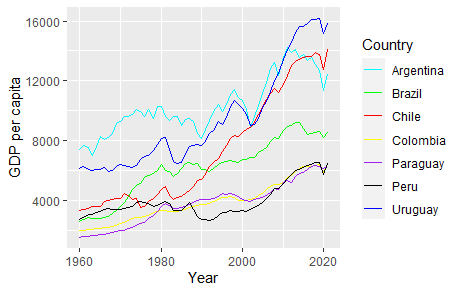
\includegraphics[scale=1.2]{images/latin_america.png}
	\end{figure}
	
	
	
	\item[\textbf{b)}] América do Norte.
	
	
	\textbf{Solução}
	
	\lstinputlisting[language=R]{codes/solution6b.R}
	
	
	\begin{figure}[H]
		\caption{América do Norte}
		\centering
		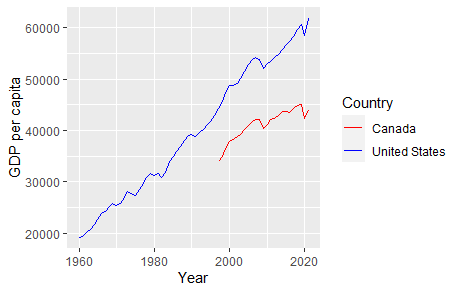
\includegraphics[scale=1.2]{images/north_america.png}
	\end{figure}
	
	
	
	\item[\textbf{c)}] Europa.
	
	
	\textbf{Solução}
	
	\lstinputlisting[language=R]{codes/solution6c.R}
	
	
	\begin{figure}[H]
		\caption{Europa}
		\centering
		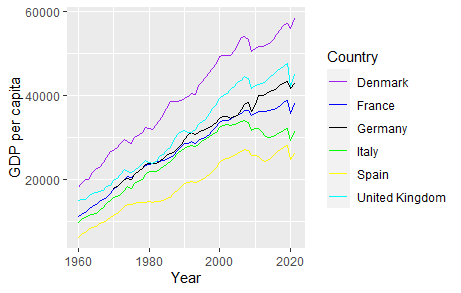
\includegraphics[scale=1.2]{images/europe.png}
	\end{figure}
	
	
	
\end{itemize}


	
\end{document}